\documentclass{ximera}

\author{Anna Davis} \title{MTH 160 Homework 2} 

\begin{document}

\begin{abstract}

\end{abstract}
\maketitle
 \textit{Certificate due: 9/2/2020 at 11:59 p.m.}
 \subsection{Lecture 2}
\begin{problem}\label{prob:160hom2prob1}
Find the domain of each function and express it in interval notation.  (Hint: type the word "infinity" to get the $\infty$ symbol.)
\begin{enumerate}
    \item $f(x)=\frac{1}{x^2}$
    $$\answer{(-\infty,0)}\cup\answer{(0,\infty)}$$
    \item $f(x)=\frac{1}{x^2-1}$
    $$\answer{(-\infty,-1)}\cup\answer{(-1,1)}\cup\answer{(1,\infty)}$$
    \item $f(x)=\frac{1}{x^2+1}$
    $$\answer{(-\infty,\infty)}$$
    \item $f(x)=\sqrt{2x-4}$
    $$\answer{[2,\infty)}$$
     \item $f(x)=\frac{1}{\sqrt{x-3}}$
    $$\answer{(3,\infty)}$$
    \item $f(x)=\frac{x+1}{(x-4)(x+7)}$
    $$\answer{(-\infty,-7)}\cup\answer{(-7,4)}\cup\answer{(4,\infty)}$$
\end{enumerate}
\end{problem}

\begin{problem}\label{prob:160hom2prob2}
  Find the range of each function and express it in interval notation.  (Hint: type the word "infinity" to get the $\infty$ symbol.)
  \begin{enumerate}
      \item $f(x)=x^2+2$
      $$\answer{[2,\infty)}$$
      \item $f(x)=-x^2$
      $$\answer{(-\infty,0]}$$
  \end{enumerate}
\end{problem}

\begin{problem}\label{prob:160hom2prob3}
Find the domain and range for each function represented graphically.
\begin{enumerate}
    \item Graph of f:
     \begin{image}
   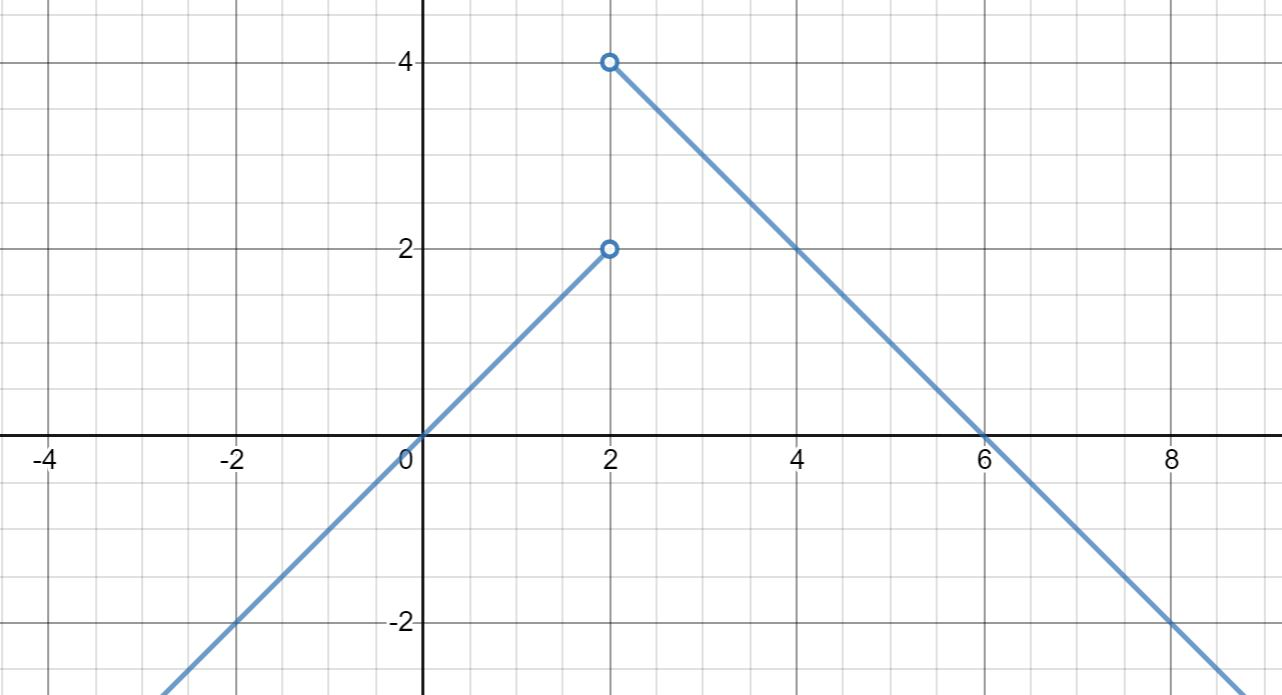
\includegraphics[height=1in]{160H2pic1.jpg}
 \end{image}
 
 Domain: $\answer{(-\infty,2)}\cup\answer{(2,\infty)}$
 
 Range:  $\answer{(-\infty,4)}$
 \item Graph of f:
     \begin{image}
   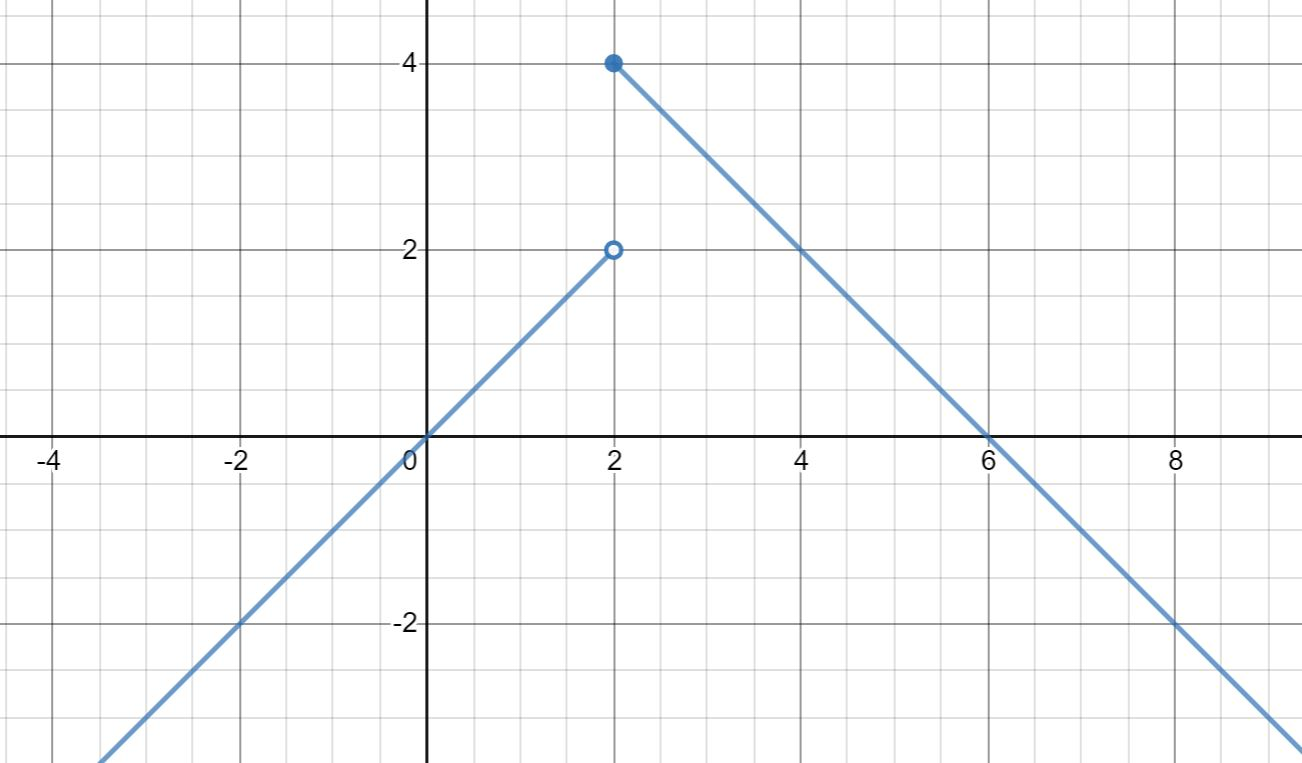
\includegraphics[height=1in]{160H2pic2.jpg}
 \end{image}
 
 Domain:$\answer{(-\infty,\infty)}$
 
 Range:  $\answer{(-\infty,4]}$
 \item Graph of f:
     \begin{image}
   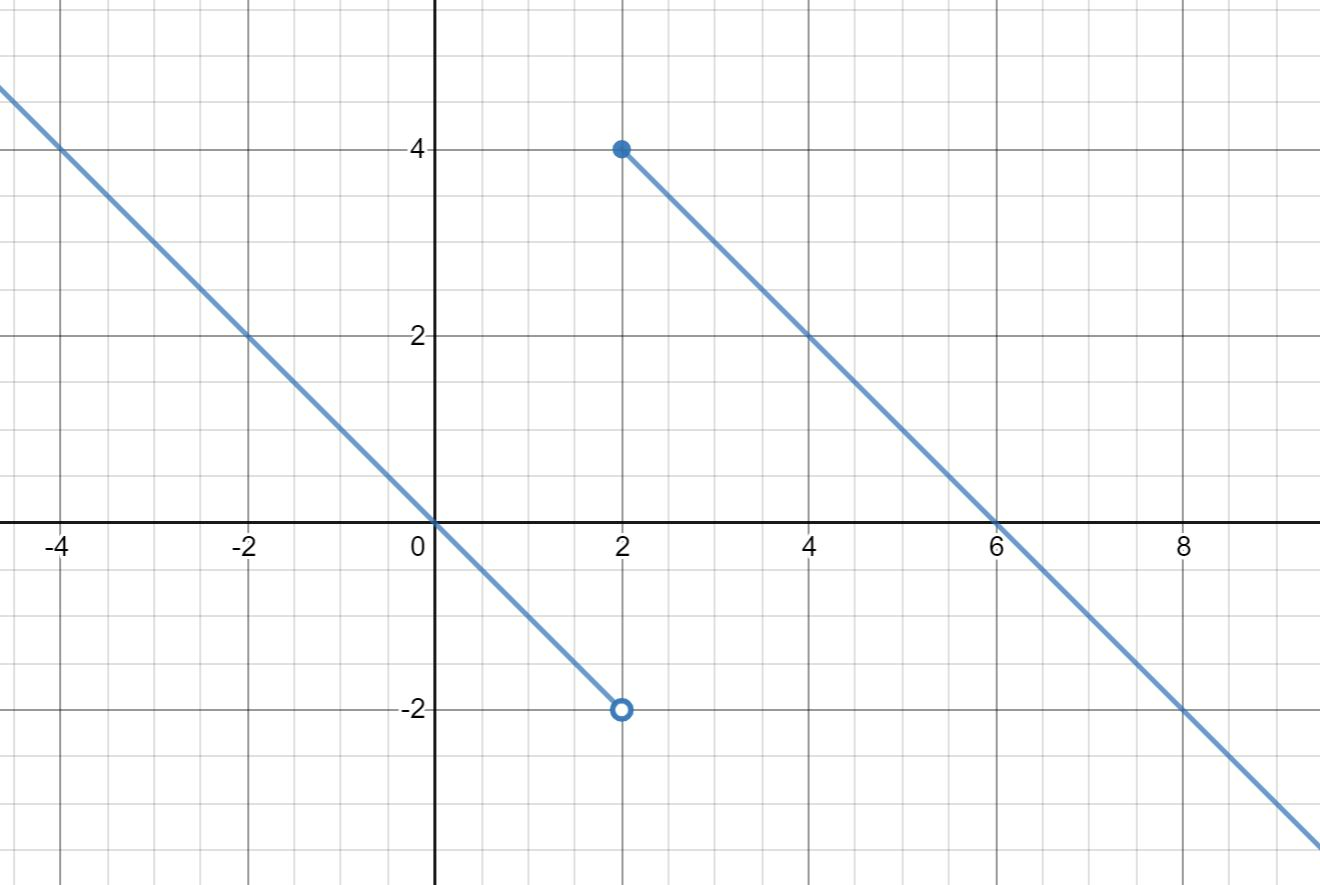
\includegraphics[height=1in]{160H2pic3.jpg}
 \end{image}
 
 Domain: $\answer{(-\infty,\infty)}$
 
 Range: $\answer{(-\infty,\infty)}$
 \item Graph of f:
     \begin{image}
   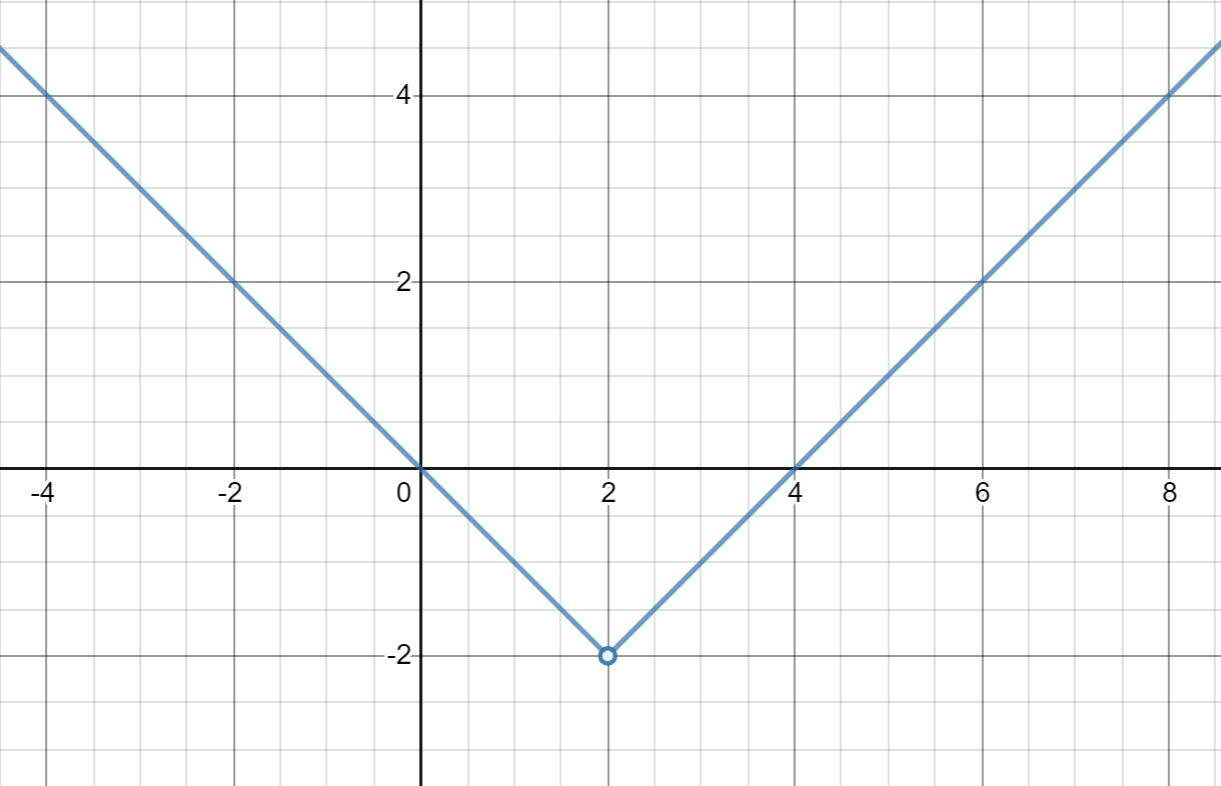
\includegraphics[height=1in]{160H2pic4.jpg}
 \end{image}
 
 Domain:  $\answer{(-\infty,2)}\cup\answer{(2,\infty)}$
 
 Range: $\answer{(-2,\infty)}$
 \item Graph of f:
     \begin{image}
   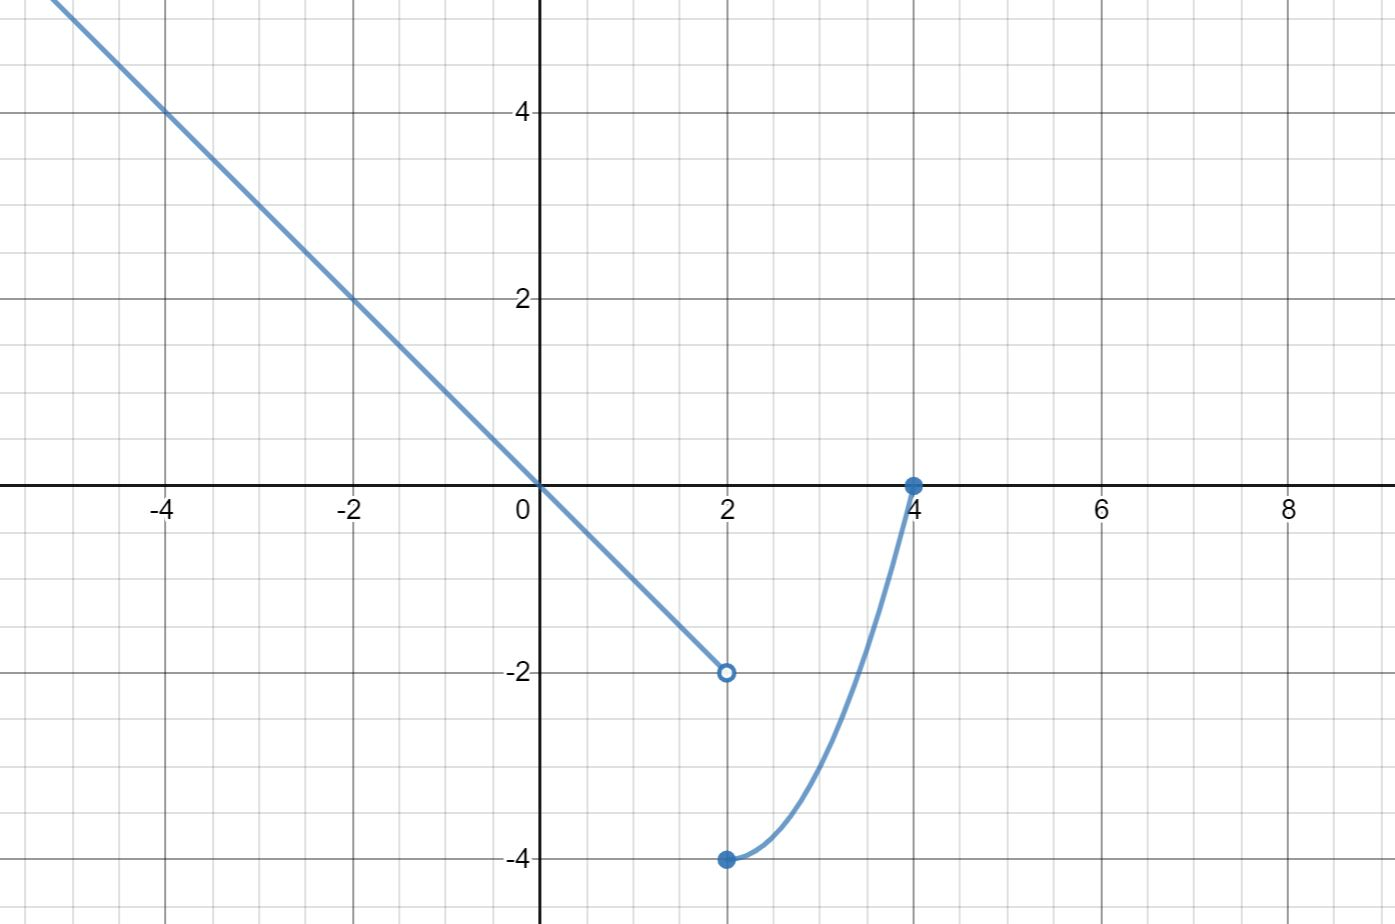
\includegraphics[height=1in]{160H2pic5.jpg}
 \end{image}
 
 Domain: $\answer{(-\infty,4]}$
 
 Range: $\answer{[-4,\infty)}$
\end{enumerate}
\end{problem}
\subsection{Lecture 3}
\begin{problem}\label{prob:160hom2prob4}

\end{problem}

\begin{problem}\label{prob:160hom2prob5}

\end{problem}

\begin{problem}\label{prob:160hom2prob6}

\end{problem}
\end{document} 